\chapter{Architecture}
\label{cha:architecture}

In order to accelerate SHA256 hashing in SHMAC, an accelerator for the SHA256 algorithm
was developed. To further increase performance, a DMA was developed to move data between
memory and the accelerator.

The new modules were then added to SHMAC in a new tile.

\section{Accelerated Hashing Tile}
\label{sec:aht}

In order to test the effects of accelerating SHA256 hashing, a new tile was developed for
SHMAC, which can be seen in figure \ref{fig:SHA-Tile}.

\begin{figure}[htb]
    \centering
    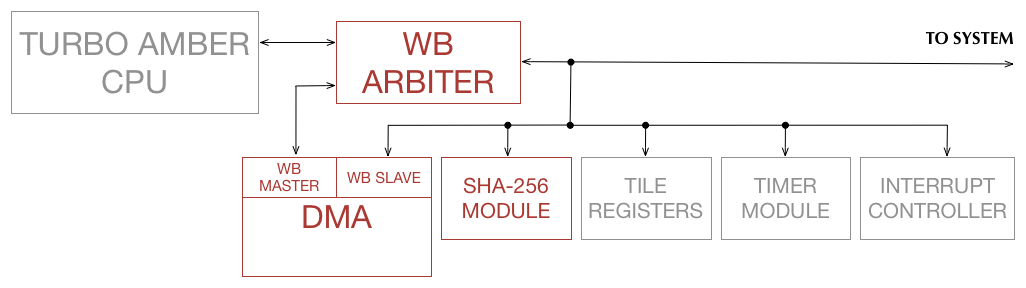
\includegraphics[width=1.0\textwidth]{Figures/Tile/HashingTile}
    \caption{SHMAC tile with SHA256 accelerator and DMA. New components are shown in red, while pre-existing components are shown in grey.}
    \label{fig:SHA-Tile}
\end{figure}

The new tile is derived from the existing CPU tile for SHMAC, the Turbo Amber tile, which contains
a ``Turbo Amber'' CPU, which is an improved version of the open-source Amber CPU, providing various
performance optimizations over the original Amber and supporting the ARMv4t instruction set \cite{turboamber}.

In addition, the tile provides two timer modules and an interrupt controller, in addition to required
tile interfaces and a router module.\todo{Consider adding this to figure?}

\subsection{SHA-256 Hashing Module}

The hashing module made for this project is a simple implementation of the algorithm described in
appendix \ref{app:hashing-algo}. It uses 65 cycles to compute the hash of its input data, running
one iteration of the SHA256 compression function every cycle except cycle 65, which is used to
form new intermediate hash values from the results of the compression function.

In order for the module to remain generic, so that it can also be used in cryptography, it
is also not optimized specifically for bitcoin mining; specifically, this means that the module
does not support doing the two-pass hashing required by the bitcoin protocol, instead relying
on software to set up correct input data for the second pass. It also relies on software to
do the neccessary padding of the input data as required by the SHA256 algorithm.

The module is controlled by the processor using a memory-mapped interface. This allows the use
of a DMA to offload data transfer between memory and the hashing module. The memory-mapped interface
provides registers for 512 bits of input and 256 bits of output data, in addition to control and
status registers. This interface can also be used for accelerators of other cryptographic hash
functions which processes input data of the same length and returns a hash of 256 bits or less,
such as RIPEMD-160 or RIPEMD-256 \cite{ripemd} or the still popular MD5 algorithm \cite{md5}.

With some work, the interface could be made even more generic in order to support algorithms
with other input and output sizes; a possibility would be to eliminate the input and output
registers completely in favour of using a DMA built into the module to move data of arbitrary
sizes into and out of the module.

Another, alternative interface to the module that was considered was using the co-processor interface
of the CPU to communicate with the module. The ARM instruction set supports up to 16 coprocessors,
which can be communicated with using the \texttt{mrc} and \texttt{mcr} instructions. Using this
interface for the hashing module would, however, have made it impossible to use a DMA to transfer
data to and from the module, making the hashing process much more dependent on the CPU, limiting
its benefits as an accelerator for offloading work from the processor.

\subsection{DMA Module}
%Originally made for the \todo{would need a reference} project during the Autumn 2014 at NTNU, the DMA Module has been modified further for use in this project.
%It can be seen in figure \ref{fig:DMATop}.

\begin{figure}[htb]
    \centering
    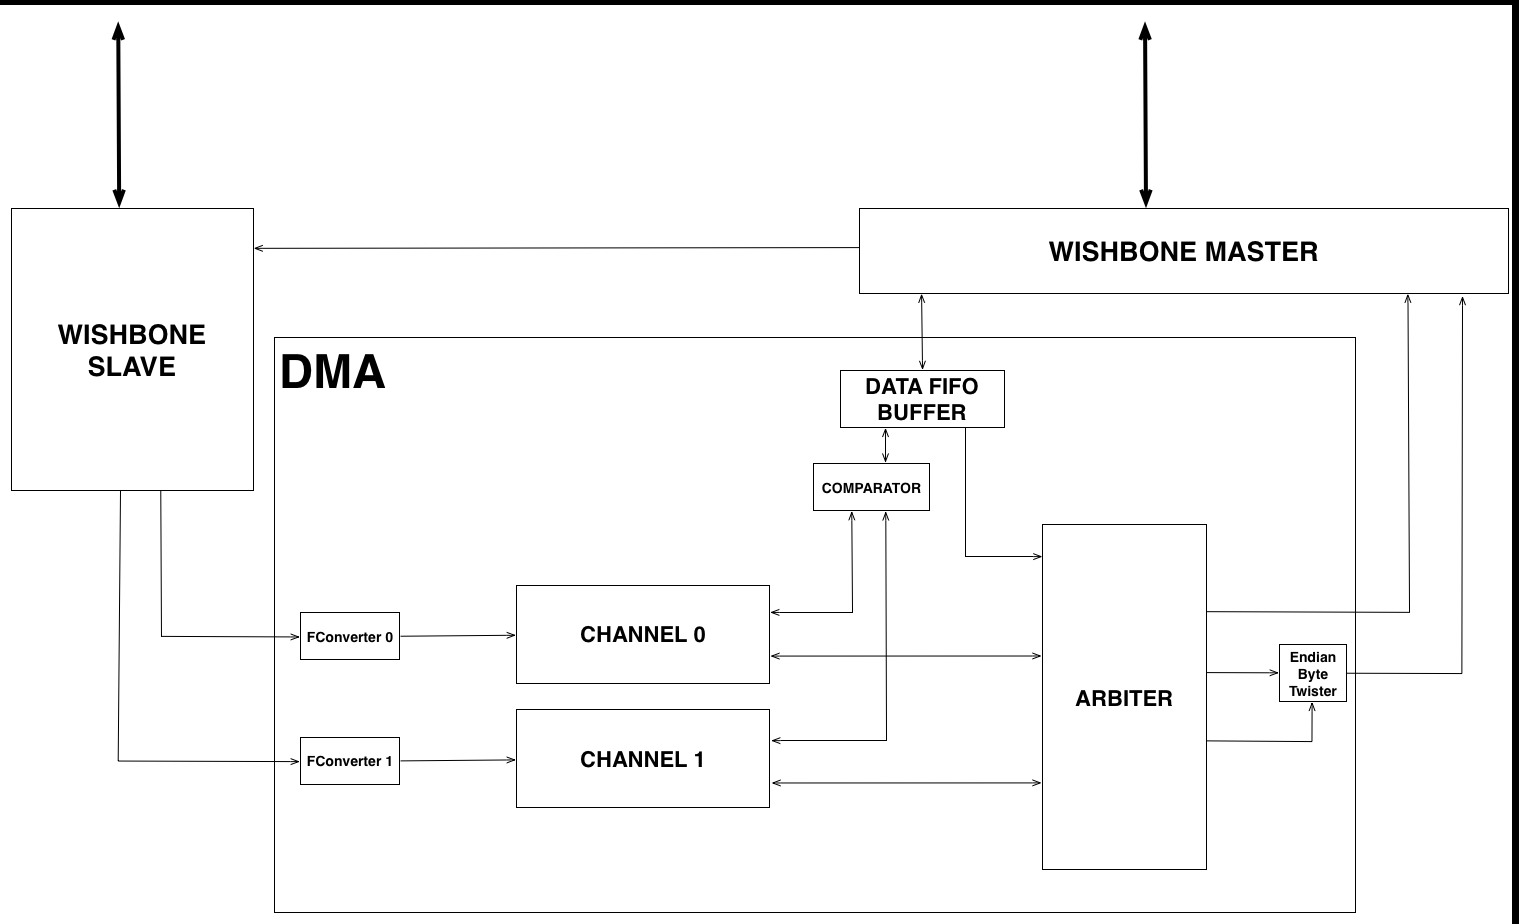
\includegraphics[width=1.0\textwidth]{Figures/DMA/DMATopview}
    \caption{DMA Topview, including Wishbone interface.}
    \label{fig:DMATop}
\end{figure}

The DMA module was made as part of the project to test if separate data transfers with a DMA module could improve performance and energy efficiency in the hashing process, freeing up the on-tile CPU for other work.

The DMA consists of a wishbone slave interface accessible for configuration, a wishbone master
interface for transferring data and the DMA module itself.

%NOTE TO SELF: The way the text is now, there is no explanation of the figure's components.
%Must keep an eye on the feedback.

%\todo{The 14th commandment: Thou shall satisfy Kristian. The 13th commandment: Thou shall satisfy ME!!!}
\todo{Hmmm... Can agree that this is a little bit nit-picky. See if this can be summed up shorter and better.}
The Wishbone Slave consists of three registers for each DMA Channel, making it six in total.
The registers are used for base source, base destination and detailing the transfer request.
When request is activated, the selected channel receives data from the slave, and executes the transfer.
An arbiter arbitrates between the channels if both are active.
Every single command, either load or store, are passed from the channels to the Wishbone master, where they are executed.
Any received data from a load command is sent on to the correct channel, and when a channel if finished, the imformation is passed from the Wishbone Master to the Wishbone Slave, so it can modify its registers and interrupt the CPU. 

In addition, the DMA supports switching the endianness of the data it copies. This improves performance
when used with the SHA256 accelerator, because the results from the accelerator are big-endian numbers
and must be converted to little-endian to be used by the software running on the processor. Converting
endianness in software adds several several additional store and arithmetic operations, which are now avoided.

\subsection{Wishbone Arbiter}
Since the DMA is a wishbone master, the CPU tile needs an arbiter to arbitrate between the DMA and the CPU
on the wishbone bus. For this purpose, the reference arbiter from the Public domain library for VHDL \cite{WBLibrary}
was adapted for use. This is a round-robin arbiter, illustrated in figure \ref{fig:WBArbiter}.

%
%For this project, the ARB0001a: 4 Level, Round-robin Arbiter from WISHBONE Public Domain Library for VHDL has been taken in use.
%Figure \cite{fig:WBArbiter} shows how the arbitration works, with Round-robin.
%The arbiter will in turn check each input master for bus requests, and grants access thereby.
%If a master has no request, the arbiter will continue to the next.
%For this project, only two masters are present.
%Arbitration normally take a full clock cycle.
%See \cite{WBLibrary} for detailed implementation.
%
\begin{figure}[htb]
    \centering
    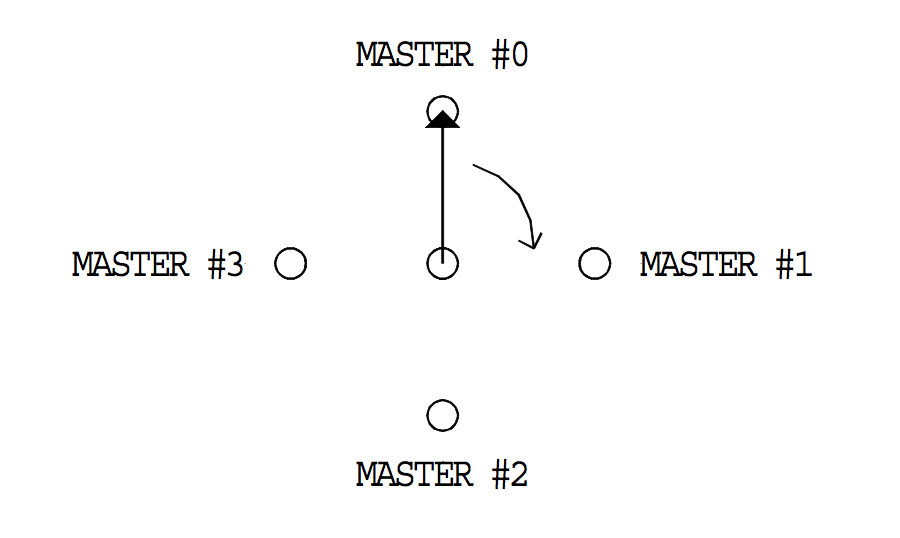
\includegraphics[width=1.0\textwidth]{Figures/Tile/WBArbiter}
    \caption{Wishbone Round-robin Arbiter, as seen in \cite{WBLibrary}.}
    \label{fig:WBArbiter}
\end{figure}

Round-robin arbiters work well in data acquisition systems where data is collected and placed into memory, since peripherals must often store data to memory. % on an equal basis.
The choice of this arbiter is because using an already established wishbone arbiter saves time as opposed to desiging a new on, which may end up less efficient in worse case.
An alternative to a round-robin arbiters is a priority arbiter.
%These are usually disadvantagous in said systems, but does not have the arbitration overhead \cite{WBLibrary}.\
\todo{Discussion of alternatives. The following may be moved to future work.}

In the case of arbitration between a CPU and a DMA module, a priority arbiter may be used to achieve either burst mode, where the DMA gets full access on the bus until the transfer is finished, or transparent mode, where the CPU always has priority on the bus.
The latter mode gives the slowest DMA transfer, but has been shown to give best overall system performance. \todo{Find those book sources again, if time. Current source does not validate claim of overall performance} \cite{DMA-lecture}.

